%fich.tex
%%%%%%%%%%%%%%%%%%%%%%%%%%%%%%%%%%%%%%%%%%%%%%%%%%%%%%%%%%%%%%%%%%%%%%%%
% Fco. Javier Bóhorquez Ogalla
% Descripción del documento:
	
%%%%%%%%%%%%%%%%%%%%%%%%%%%%%%%%%%%%%%%%%%%%%%%%%%%%%%%%%%%%%%%%%%%%%%%%


%%%%%%%%%%%%%%%%%%%%%%%%%%%%%%%%%%%%%%%%%%%%%%%%%%%%%%%%%%%%%%%%%%%%%%%%
%Clase de documento
\documentclass[12pt, spanish]{article}
%%%%%%%%%%%%%%%%%%%%%%%%%%%%%%%%%%%%%%%%%%%%%%%%%%%%%%%%%%%%%%%%%%%%%%%%


%%%%%%%%%%%%%%%%%%%%%%%%%%%%%%%%%%%%%%%%%%%%%%%%%%%%%%%%%%%%%%%%%%%%%%%%	
%Paquetes de lenguaje:
%%%%%%%%%%%%%%%%%%%%%%%%%%%%%%%%%%%%%%%%%%%%%%%%%%%%%%%%%%%%%%%%%%%%%%%%
\usepackage[utf8]{inputenc}
\usepackage[spanish]{babel}
%\usepackage[spanish, activeacute] {babel}	
%\usepackage[spanish]{babel} 				
%\usepackage[latin1]{inputenc}
%%%%%%%%%%%%%%%%%%%%%%%%%%%%%%%%%%%%%%%%%%%%%%%%%%%%%%%%%%%%%%%%%%%%%%%%


%%%%%%%%%%%%%%%%%%%%%%%%%%%%%%%%%%%%%%%%%%%%%%%%%%%%%%%%%%%%%%%%%%%%%%%%
%Paquetes para encabezados y pie de páginas
%%%%%%%%%%%%%%%%%%%%%%%%%%%%%%%%%%%%%%%%%%%%%%%%%%%%%%%%%%%%%%%%%%%%%%%%
\usepackage{fancyhdr}
%%%%%%%%%
% \pagestyle{fancy} %Si se cambia el estilo de página, antes de empezar 
	%el documento. Esto hace que el emcabezado y pie de página se 
	%quede separado del texto por una línea
%%%%%%%%%	
% \fancyhead{} % Límpia el texto que se está usando como encabezado
%%%%%%%%%
% \fancyhead[OPCIONES]{Encabezado}
	% OPCIONES:
		% L texto a la izquierda
		% C texto centrado
		% R texto a la derecha
		% E página par
		% O pagina impar
	%Ejemplo: 
		% fancyhead [LE] {"Doc. Latex"} 
			% Establece como emcabezado de las páginas pares "Doc Latex"
			% con alineacion a la izquierda
%%%%%%%%%			
% \fancyfoot[OPCIONES]{Píe de pag.}
	% OPCIONES:
		% L C R E O
	%Ejemplo
		% \fancyfoot[LE,RO]{\thepage} 
			% Establece como píe de pág. el número de página. con 
			% alineación a la izq en paginas pares y a la derecha en
			% las impares
%%%%%%%%%			
% \renewcommand{\headrulewidth}{0.4pt}
% \renewcommand{\footrulewidth}{0.4pt}
	% Fija el grosor de la la linea que separa el emcabezado y pie de pág
%%%%%%%%%
% Otros comandos:
%\lhead{}
%\chead{}
%\rhead{}
%\lfoot{}
%\cfoot{}
%%%%%%%%%%%%%%%%%%%%%%%%%%%%%%%%%%%%%%%%%%%%%%%%%%%%%%%%%%%%%%%%%%%%%%%%


%%%%%%%%%%%%%%%%%%%%%%%%%%%%%%%%%%%%%%%%%%%%%%%%%%%%%%%%%%%%%%%%%%%%%%%%
% Paquetes para tamaños y distancias
%%%%%%%%%%%%%%%%%%%%%%%%%%%%%%%%%%%%%%%%%%%%%%%%%%%%%%%%%%%%%%%%%%%%%%%%
\usepackage{anysize} 
%%%%%%%%%%%
% \marginsize{3cm}{2cm}{2cm}{2cm}
	% Controla los márgenes {izquierda}{derecha}{arriba}{abajo}. 
%%%%%%%%%%%%%%%%%%%%%%%%%%%%%%%%%%%%%%%%%%%%%%%%%%%%%%%%%%%%%%%%%%%%%%%%


%%%%%%%%%%%%%%%%%%%%%%%%%%%%%%%%%%%%%%%%%%%%%%%%%%%%%%%%%%%%%%%%%%%%%%%%
%Paquetes de carácteres especiales:
%%%%%%%%%%%%%%%%%%%%%%%%%%%%%%%%%%%%%%%%%%%%%%%%%%%%%%%%%%%%%%%%%%%%%%%%
\usepackage{dsfont}	
%Para representar conjuntos matematicos comunes: Z, N, R...
	% mathds{R}, mathds{N},...
%%%%%%%%%%%%%%%%%%%%%%%%%%%%%%%%%%%%%%%%%%%%%%%%%%%%%%%%%%%%%%%%%%%%%%%%

%%%%%%%%%%%%%%%%%%%%%%%%%%%%%%%%%%%%%%%%%%%%%%%%%%%%%%%%%%%%%%%%%%%%%%%%
%Paquetes para insertar gráficos
%%%%%%%%%%%%%%%%%%%%%%%%%%%%%%%%%%%%%%%%%%%%%%%%%%%%%%%%%%%%%%%%%%%%%%%%
\usepackage[dvips]{graphicx}
\DeclareGraphicsExtensions{.pdf,.png,.jpg} %solo para PDFLaTeX
%%%%%%%%%%%%%%%%%%%%%%%%%%%%%%%%%%%%%%%%%%%%%%%%%%%%%%%%%%%%%%%%%%%%%%%%

%%%%%%%%%%%%%%%%%%%%%%%%%%%%%%%%%%%%%%%%%%%%%%%%%%%%%%%%%%%%%%%%%%%%%%%%
%Paquetes de color:
%%%%%%%%%%%%%%%%%%%%%%%%%%%%%%%%%%%%%%%%%%%%%%%%%%%%%%%%%%%%%%%%%%%%%%%%
\usepackage{color}
%%%%%%%%%%%%%%%%%%%%%%%%%%%%%%%%%%%%%%%%%%%%%%%%%%%%%%%%%%%%%%%%%%%%%%%%
%Definición de colores:
\definecolor{gray97}{gray}{.97}
\definecolor{gray75}{gray}{.75}
\definecolor{gray45}{gray}{.45}
%%%%%%%%%%%%%%%%%%%%%%%%%%%%%%%%%%%%%%%%%%%%%%%%%%%%%%%%%%%%%%%%%%%%%%%%


%%%%%%%%%%%%%%%%%%%%%%%%%%%%%%%%%%%%%%%%%%%%%%%%%%%%%%%%%%%%%%%%%%%%%%%%
%Paquete de listado de código:
%%%%%%%%%%%%%%%%%%%%%%%%%%%%%%%%%%%%%%%%%%%%%%%%%%%%%%%%%%%%%%%%%%%%%%%%
\usepackage{listings}
%%%%%%%%%%%%%%%%%%%%%%%%%%%%%%%%%%%%%%%%%%%%%%%%%%%%%%%%%%%%%%%%%%%%%%%%
%Configuración del listado:
\lstset { 
	frame=Ltb,
     framerule=0pt,
     aboveskip=0.2cm,
     framextopmargin=0.3pt,
     framexbottommargin=0.2pt,
     framexleftmargin=0.3cm,
     framesep=0pt,
     rulesep=.1pt,
     tabsize=2,
     backgroundcolor=\color{gray97},
     rulesepcolor=\color{black},
     %
     stringstyle=\ttfamily,
     showstringspaces = false,
     basicstyle=\scriptsize\ttfamily,
     commentstyle=\color{gray45},
     keywordstyle=\bfseries,
   	%
     numbers=left,
     numbersep=1pt,
     numberstyle=\tiny,
     numberfirstline = false,
     breaklines=true,
}
%%%%%%%%%%%%%%%%%%%%%%%%%%%%%%%%%%%%%%%%%%%%%%%%%%%%%%%%%%%%%%%%%%%%%%%%


%%%%%%%%%%%%%%%%%%%%%%%%%%%%%%%%%%%%%%%%%%%%%%%%%%%%%%%%%%%%%%%%%%%%%%%%
%Indexado. Índice alfabeticos
\usepackage{makeidx}
\makeindex %para habilitar indices
%%%%%%%%%%%%%%%%%%%%%%%%%%%%%%%%%%%%%%%%%%%%%%%%%%%%%%%%%%%%%%%%%%%%%%%%
%Forma de uso:
% \index{clave} %Para crear un indice de materia
% Supongase que queremos meter en el indice alfabetico referencias a 
% las paginas donde se hace referencia a la clave Producto escalar
% en tal caso en cada una de las páginas pondremos \index{Producto escalar}
% \printindex %Para imprimir el índice alfabetico

% Es necesario una doble compilación del documento. La primera genera un 
% fichero.idx el cual tendremos que procesar con la aplicación makeindex
%tras procesarlo se creará un fichero.ind que contendra el código Latex 
% que se inserta en el documento original. 
% Tras la segunda compilación del documento original se sustituira el
% comando \printindex por el contenido del fichero.ind 

%Podemos cambiar el formato de la clave:
%Ejemplo     				&    	Entrada 		&	Comentario
%\index{hola}				&         hola, 1   	&	Entrada simple
%\index{hola!Pedro}			&		 Pedro, 3 	&	Subentrada bajo ‘hola’
%\index{Juan@\textsl{Juan}}  	&		Juan, 2    	&	Entrada con diseño                        
%\index{Pepa@\textbf{Pepa}}	&		Pepa, 7    	&	Igual que antes
%\index{Loli|textbf}		&		Loli, 3    	&	No de página con diseño                     
%\index{Soraya|textit}		&		Soraya, 5  	&	Igual que antes
%%%%%%%%%%%%%%%%%%%%%%%%%%%%%%%%%%%%%%%%%%%%%%%%%%%%%%%%%%%%%%%%%%%%%%%%


%%%%%%%%%%%%%%%%%%%%%%%%%%%%%%%%%%%%%%%%%%%%%%%%%%%%%%%%%%%%%%%%%%%%%%%%


%%%%%%%%%%%%%%%%%%%%%%%%%%%%%%%%%%%%%%%%%%%%%%%%%%%%%%%%%%%%%%%%%%%%%%%%
%Estilo de página
%%%%%%%%%%%%%%%%%%%%%%%%%%%%%%%%%%%%%%%%%%%%%%%%%%%%%%%%%%%%%%%%%%%%%%%%
%\textwidth 6.75in								  %ancho de texto
%\oddsidemargin -0.2in							%margen izquierdo 
\parskip 0.2in									%espacio parrafos
%%%%%%%%%%%%%%%%%%%%%%%%%%%%%%%%%%%%%%%%%%%%%%%%%%%%%%%%%%%%%%%%%%%%%%%%

\usepackage{titlesec}

\setcounter{secnumdepth}{4}

\titleformat{\paragraph}
{\normalfont\normalsize\bfseries}{\theparagraph}{1em}{}
\titlespacing*{\paragraph}
{0pt}{3.25ex plus 1ex minus .2ex}{1.5ex plus .2ex}


%%%%%%%%%%%%%%%%%%%%%%%%%%%%%%%%%%%%%%%%%%%%%%%%%%%%%%%%%%%%%%%%%%%%%%%%	
%datos del documento
\author{Fco. Javier Bohórquez Ogalla}						%autor
\date{}														%fecha

\title{Ilos}
%%%%%%%%%%%%%%%%%%%%%%%%%%%%%%%%%%%%%%%%%%%%%%%%%%%%%%%%%%%%%%%%%%%%%%%%

%%%%%%%%%%%%%%%%%%%%%%%%%%%%%%%%%%%%%%%%%%%%%%%%%%%%%%%%%%%%%%%%%%%%%%%%
%Documento:
%%%%%%%%%%%%%%%%%%%%%%%%%%%%%%%%%%%%%%%%%%%%%%%%%%%%%%%%%%%%%%%%%%%%%%%%
\begin{document}
\maketitle
\pagebreak
\tableofcontents
\pagebreak
\section{Introducción}
Gran parte de la información que llega a las casas modernas lo hace a través de una computadora
conectada a internet. La máquina pasa a formar parte de una red de comunicación a escala mundial constituida por
una inmensa cantidad y diversidad de computadoras o sistemas informáticos. Internet es un espacio no centralizado que ofrece multitud de servicios
y que está en constante cambio.

Uno de los servicios que nos ofrece la tecnología que representa internet es la World Wide Web. La web se define como un sistema 
distribuido de documentos que contienen información en diversas formas y que, generalmente, enlazan a otros documentos. Estos documentos 
son denominados comúnmente como páginas web.  

Los servicios web representan aquellos servicios que se ofrecen mediante el sistema de documentos que representa la World Wide Web, concretamente
mediante la tecnología que la hace posible, el protocolo de la capa de aplicación HTTP. Estos servicios son prestados por sistemas informáticos 
denominados servidores web. Un servidor web pone a disposición del agente, cliente o usuario información en forma de documento web. La mayoría de estos servicios
esperan ser consumidos por una persona que haga uso de un software denominado navegador web. No obstante también 
existen servicios pensados para ser consumidos por otros programas informáticos. 

Un documento web puede estar escrito en varios lenguajes, cada uno de los cuales tendrá un propósito. Cuando el destinatario del documento es una persona en un navegador web 
lo más común es que se utilice un lenguaje de marcado para dar estructura a la información, acompañado de lenguajes de estilo para definir la presentación y el formato, o lenguajes de 
programación para dotar de funcionalidad e interactividad al documento. En este caso es el navegador web el encargado de interpretar el documento. Cuando el destinatario del documento
es otra aplicación lo normal es utilizar lenguajes que definan la estructura e incluso el significado semántico de los datos. 

Además de los servicios web en internet existen una gran cantidad de servicios que operan con distintos protocolos: FTP, SSH, TELNET... Cada servicio 
suele estar pensado para un software cliente específico.

Ilos es un proyecto software que nace del deseo de aprovechar los servicios de red de una forma automática, fácil y personalizada, con independecia del destinatario 
para el que fue construido el servicio. Persige el ofrecer mayor control sobre los servicios de internet y la información ofrecida por estos.

En el presente documento se hará una presentación al sistema software Ilos. 

\section{Definición y características de Ilos}
Ilos (Interpreted Language of Operation of Services) es un lenguaje de programación completo y de alto nivel. 
Aunque bien puede ser utilizado para un propósito general es un lenguaje específico del dominio de la explotación 
de servicios de red. En este contexto se entiende por explotación como la obtención de un beneficio ligado al servicio, como podría ser la 
ejecución de una determinada tarea o la obtención de una serie de datos. 

Ilos presenta mecanismo para la comunicación con el servicio, además facilita la manipulación, 
el almacenamiento y la presentación de los datos obtenidos. 

Es un lenguaje interpretado por lo que las intrucciones que conforman un programa Ilos son traducidas y ejecutadas 
en tiempo de ejecución por un software denominado intérprete. Ilos se puede considerar un lenguaje de scripts pues, además de ser interpretado, sus instrucciones pueden ser 
ejecutadas una a una por un operador humano.

Según la manera de abordar la tarea a realizar Ilos se puede ver como un lenguaje de programación imperativo, ya que todo 
programa representa un conjunto de instrucciones que cambian el estado del mismo e indican cómo realizar 
una determinada tarea. Sin embargo, en lo referente a la explotación de un determinado servicio, Ilos se 
podría ver como un lenguaje declarativo, ya que en cierto modo indica qué se quiere obtener del servicio y no cómo obtenerlo. 

Respecto al estilo de programación que se puede seguir cuando se escribe un programa, este puede atender a un paradigma 
funcional, organizando conjuntos de intrucciones en funciones o procedimientos con un proposito determinado. También puede
presentar características propias de los lenguajes orientados a objetos, como la definición de clases, herencia...

Para modelar ciertos aspectos de la comunicación con el servicio web presenta características de los lenguajes para defenir ontologías. 
Un programa Ilos puede definir el significado semántico de los datos obtenidos de un servicio web. 

A pesar de ser un lenguaje con el propósito de explotar servicios web, Ilos no es un lenguaje pensado para el desarrollo de sistemas distribuidos. Por lo general 
un programa ve el servicio web como un actor externo al propio sistema. No obstante es posible utilizar Ilos para desarrollar 
sistemas o componentes de carácter distribuido, por ejemplo servicios web que se comunican unos con otros.

Ilos es un lenguaje con una gramática y semántica extensible, es posible añadir nuevas características al lenguaje mediante módulos. Además posee un gramática personalizable 
en cierto grado, en el sentido de que muchas palabras claves del lenguaje poseen una abreviación editable por el programador. Esto hace de él un lenguaje más cercano al 
desarrollo de aplicaciones personales que premia la rapidez y sencillez en el proceso.

Este lenguaje es débilmente tipificado, es decir, no realiza una comprobación estricta de tipos datos.

Otra característica de este lenguaje formal es que su gramática permite expresar concurrencia, pudiendose llevar a cabo la ejecución simultánea 
de múltiples tareas o procesos. Además es un lenguaje de programación determinista dado que en todo programa Ilos a partir de un estado o entrada se puede predecir el 
siguiente estado o salida.  

\section{Lenguaje completo y de alto nivel}
Ilos es un lenguaje Turing completo. Esto quiere decir que su poder computacional es equivalente a una máquina universal de Turing. 

Un programa escrito en Ilos conciste en una serie de sentencias o instrucciones que normalmente serán interpretadas y ejecutadas de forma secuencial. 
El lenguaje ofrece mecanismos para leer y escribir diferentes tipos de datos en un espacio de memoria. También pone a disposición una 
serie de operadores aplicables a estos datos. Ilos incorpora  estructuras de control para alterar el orden secuencial en el que se ejecuta el programa. Además permite la definición
y uso de estructuras organizativas y funcionales como las subrutinas o las clases de objetos.    

Ilos es además un lenguaje de alto nivel dado que muchas de las instrucciones que ofrece representa un alto grado de abstracción. Una instrucción en Ilos
se traduce como muchas instrucciones en lenguaje máquina. Además una sola instrucción en lenguaje Ilos puede resolver un problema complejo y con un 
nivel conceptual alto como realizar una solicitud a un servicio o escribir en un fichero.

\subsection{Instrucciones}
Una instrucción o sentencia Ilos es una expresión escrita con el léxico y las reglas de sintáxis pertenecientes a este lenguaje. Toda instrucción puede ser 
interpretada y ejecutada, produciendo así un resultado o cambio de estado. Las instrucciones tienen un significado semántico ligado que se representa mediante la ejecución de un 
determinado conjunto de tareas. Una instrucción Ilos conciste en una expresión que contiene operadores, datos y otros elementos del lenguaje que puede ser
interpretada y ejecutada.

Mediante una serie de instrucciones Ilos se pueden expresar algoritmos. Un programa Ilos conciste en 
un conjuto estructurado de instrucciones que modelan algoritmos que dan solución a un problema o conjunto de estos. Estos problemas se 
corresponden con las necesidades de una serie de requisitos funcionales.

Las instrucciones se pueden organizar en bloques, formando estructuras con un determinado significado. El bloque se ve como una única instrucción y su 
ejecución dependerá de la naturaleza y significado de la sentencia de bloque.

Una instrucción que representa una expresión Ilos puede conllevar la ejecución de varias tareas. Para interpretar una sentencia primero se realiza un análsis 
léxico, tomando cada vocablo de la expresión y constituendo los componentes léxicos o tokens asociados (unidad de información con significado para el lenguaje).
Luego se aplican una serie de reglas sintácticas sobre los componentes léxicos para construir un árbol de ejecución o semántico. Este árbol estará
formado por nodos que representan los distitnos operadores, datos y demás elementos del lenguaje presentes en la instrucción. Cada nodo tendrá asociada una única tarea 
que se llevará a cabo cuando se ejecute. Además cada nodo tomará un valor tras su ejecución. La ejecución del árbol comienza con el nodo raiz. La ejecución de un nodo generalmente
conciste en ejecutar cada uno de sus hijos, realizar una serie de operaciones con los valores que han tomado y tomar su propio valor. El programa en su totalidad se puede ver 
como un único árbol de ejecución.

\subsection{Tipos de datos}
Una instrucción puede implicar la manipulación de una serie de datos. Estos datos pueden estar definidos y 
codificados en la propia instrucción, en cuyo caso son denominados datos literales. También pueden pertenecer al conjunto de datos 
generados por la ejecución de las instrucciones anteriores, denominándose en este caso datos variables. 

Los tipos de datos que puede manipular un programa escrito en Ilos son de diversa naturaleza, complejidad y abstracción conceptual. Así se
pueden organizar de la siguiente forma: 

\subsubsection{Datos simples}
Los tipos de datos simples son aquellos tipos básicos, bien definidos en cuanto a su naturaleza y que ocupan un espacio en memoria fijo. Son tipos nucleares que 
no se derivan de otros tipos. Ilos solo reconoce tres tipos de datos simples:

\begin{itemize}
\item Booleanos: Admiten los valores true o false
\item Numéricos: Admite valores positivos desde 3.4E-4932 a 1.1E4932, y negativos desde -3.4E-4932 a -1.1E4932
\item Caracteres: Admite cualquier carácter representado por un símbolo del código ASCII.
\end{itemize}

\subsubsection{Datos compuestos}
En Ilos es posible definir un conjunto estructurado de datos simples, representado así lo que se denomina
tipo de dato compuesto. Los datos de este tipo ocupan una cantidad variable de memoria. Se proporcionan mecanismo para
manipular y operar con estos datos como un todo. En Ilos existen los siguientes tipos de datos compuestos:

\begin{itemize}
\item Cadena de caracteres: Representa un conjunto ordenado de caracteres. 
\item Expresiones regulares: Se definen como una secuencia de caracteres que forman un patrón de búsqueda
\item Diccionarios: Se ven como un conjunto de claves únicas asociadas con valores. 
Tanto las claves como los valores pueden ser de cualquier otro tipo de dato, incluso otros diccionarios.
Un diccionario con claves numéricas consecutivas desde 0 a n se denomina vector. Se suele utilizar 
el término vector asociativo para referirse a los diccionarios.
\end{itemize}

Además de estos tipos de datos básicos, Ilos define algunos tipos de datos más abstractos
que derivan de estos: ficheros, conexiones...

\subsection{Conversión de tipos}
El lenguaje de programación Ilos dota de significado semántico a los datos según la instrucción que se ejecute. 
Ilos realizará una conversión de un tipo de dato a otro siempre que sea necesario y no se indique lo contrario. 

Por ejemplo, una cadena de caracteres que presente el formato correcto para ser considerada como un dato numérico puede ser tratada 
como un dato de este tipo si es necesario. 

\subsection{Operadores y funciones del lenguaje}
Ilos define una serie de operadores. Estos relacionan elementos de un conjunto de datos inicial con los de un conjunto final. Los datos pueden ser de distinto tipo.
Los elementos del conjunto inicial se denominan operandos, y los elementos del conjunto final resultados. Al acto de aplicar el operador sobre los operandos 
se le denomina operación. 

Ilos amplia el concepto de operador defininiendo funciones propias del lenguaje que aceptan unos datos de entrada y produce un 
resultado o datos de salida. El uso de una función del lenguaje en una expresión Ilos indica que esta se ha de aplicar
a unos datos de entrada dados.

La ejecución de una operación o función conciste en la aplicación de un determinado algoritmo sobre los operandos para obtener los resultados.
En Ilos existen funciones que, dado unos datos del conjunto inicial, no los relacionan con datos del conjunto final. En este sentido se considera que las 
distintas aplicaciones del algoritmo forma el conjunto final y la función relaciona los elementos iniciales con la aplicación concreta del algoritmo. 
También es posible que el conjunto de elementos iniciales sea vacío en cuyo caso el conjunto final solo será de un sólo elemento.

El número de datos del conjunto inicial que admite un operador determina la carnalidad de este. Así es posible encontrar opeardores unitarios, binarios, ternarios...

Una instrucción Ilos puede partir de una operación o función cuyos operandos pueden ser datos directos o el resultado de aplicar otras operaciones o funciones. Se establece 
pues unas reglas de prioridad que determinan el orden en que se resolverán. 

En Ilos existe gran cantidad de operadores y funciones que se pueden clasificar según los datos de salida y el resultado producido:

\begin{itemize}
\item Asignación
\item Booleanos
\item Aritméticos
\item Cadenas
\item Expresiones regulares
\item Acceso a recursos: Diccionarios, Ficheros, Bases de datos...
\end{itemize}


\subsection{Variables}
Para acceder a los datos en memoria se utilizan variables. Las variables son referencias a los datos que son generados 
y manipulados por el programa Ilos en ejecución. Una variable se representa mediante un identificador formado por cualquier combinación 
de letras, dígitos númericos y caracteres '\_', con la restricción que no puede comenzar por un número. 

En Ilos no es necesario declarar el tipo de una variable dado que este viene determinado por la propia naturaleza del dato. Además las 
variables presentan un tipado dinámico, es decir, su tipo cambia según los datos a los que referencie

Dos o más variables pueden referenciar al mismo dato en memoria.  

Las variables, además de poder referenciar datos en memoria, también puede hacer referencia a bloques de código de la aplicación. 
Así una variable puede referenciar, por ejemplo, a la definición de una función.   

Ilos dispone de una serie de palabras reservadas que representan funciones, directivas y otros elementos del lenguaje. Estas palabras 
reservadas no pueden ser utilizadas como nombre de variables.

\subsection{Estructuras de control}
Las estrucutras de control representan un mecanismo para alterar la secuencia de ejecución de un programa. Las estructuras de control son bloques
de sentencias que no se ejecutarán de la forma secuencial habitual. 

Las estructuras de control condicionales o de selección, ejecutan un bloque de instrucciones u otro según se cumpla o no una condición. En Ilos
solo se definen las siguientes:

\begin{itemize}
\item If-Then-Else: Representa la estructura condicional más simple. De acuerdo a una condición, se ejecuta un grupo u otro de sentencias. Es posible 
omitir el bloque Else. 
\item Select-Case: Según el valor de una expresión se ejecuta un bloque determinado.
\end{itemize}

Las estructuras de control iterativas ejecutan un bloque de sentencias un número determinado de veces mientras se cumpla una condición. En Ilos se definen
las siguientes:

\begin{itemize}
\item Do-While: Ejecuta un bloque de sentencias mientras se cumpla una condición
\item For-Next: Piermite ejecutar un bloque de sentencias un número determinado de veces.
\end{itemize}

En Ilos existen otros mecanismos que, aunque no son estructuras de control, modifica el flujo de ejecución del programa:
return, break, include, goto...

\subsection{Funciones}

Además de definirse funciones propias del lenguaje, Ilos ofrece mecanismos para definir funciones como un bloque de instrucciones 
que pueden ser ejecutado desde cualquier otra instrucción del código. Las funciones pueden recibir unos parámetros de entrada y devolver un solo dato de salida.

Una función se define medinate un identificador, una lista de parámetros y un bloque de instrucciones. La lista de parámetros representa el nombre de las 
variables que van a referenciar a los datos de entrada cuando se ejecute el bloque de código. 

En una expresión Ilos se puede indicar la ejecución de una funcion medienate su identificador y una lista de datos o referencias 
a estos que serán pasados como parámetros de la función. Ha este acto se le denomina "realizar una llamada a la función". El valor que 
tome la expresión viene determinado por la ejecución del bloque de código
correspondiente a la función. Ilos proporciona un mecanismo denominado return que termina la ejecución de la función y le da un valor.

Es posible pasar como parámetros en la llamda a una función el valor que toma la ejecución de otras funciones, expreciones, variables o datos.

Los parámetros de una función se pueden pasar por referencia o por valor. Mientras que por referencia se operará sobre el dato en memoria directamente, si se 
pasa por valor el dato será duplicado y se operá con la copia. En el primer caso el elemento pasado debe ser una variable o cualquier 
otro mecanismo de acceso a memoria de ejecución.

Los parámetros de una función pueden tener valores por defecto, de forma que si no se le corresponde un dato en la llamada toma el este valor. 

Toda variable utilizada en el bloque de instrucciones de una función por defecto es local a la misma, en el sentido de que su visibilidad y duración están muy
a esta. No obstante en Ilos es posible declarar una variable como global haciendo que su visibilidad y duración sea para toda la aplicación.

\subsection{Clases de objetos}

En Ilos se puede desarrollar software que atiende al paradidgma de la programación orientada a objetos. Modelando el dominio del problema
mediante objetos que se relacionan entre si, y que encapsulan funcionalidades y datos. 

En Ilos un objeto se ve como un dato de tipo diccionario el cual tiene claves cuyo valores son funciones (métodos) y otras que son datos (atributos).
Desde una función refernciada por una clave se puede acceder de forma local  a los demás valores del diccionario contenedor. Así en Ilos es posible declarar
y utilizar un objeto directamente.También es posile declarar una clase objetos definiendo un diccionario base destinado ha ser copiado y modificado.

Ilos facilita un operador para la duplicación de una clase e inicialización del objeto resultante. Este operador indica que se ha de realizar una copia
del objeto base que representa la clase y ejecutar un método especial denominado constructor. 

Es posible definir métodos o atributos de una clase como estáticos. En el caso de un atributo esto hará que al duplicarse para generar un objeto se cree 
una referencia al dato en vez de una copia. Para acceder a cualquier miembro estático se usa la clase.  

Ilos presenta mecanismo para la herencia, lo que hace posible definir clases de objetos a partir de otras. La clase derivada o hija extenderá la definición 
de la clase base o padre. Una clase puede extender a varias clases padres permitiéndose así la herencia múltiple. 

Al ser un lenguaje débilmente tipificado el polimorfismo es posible.  

\section{Explotación de servicios}
Ilos es un lenguaje de programación orientado a la explotación de servicios de red. Así, un programa escrito en este lenguaje generalmente hará uso de 
algún servicio basado en un protocolo de internet y que esté definido en la capa de aplicación. El programa Ilos ve al servicio como un sistema ajeno con el que 
se ha de comunicar. El servicio ve a la aplicación como cualquier otro agente para el que fue diseñado.

Para poder explotar un servicio se ha de establecer una comunicación. Además la comunicación ha de ser efectiva, 
en el sentido de que se puedan otorgar un significado semántico a los datos obtenidos. Mediante Ilos se puede modelar y llevar a cabo la comunicación 
con un determinado servicio de red.

La comunicación se modela mediante estructuras de diccionarios que describen el protocolo que se utilizará, la configuración de este, los datos que se enviarán, 
y una serie de reglas sintácticas y semánticas para interpretar los datos obtenidos. Ilos proporcionará mecanismos para que, a partir de estas declaraciones, 
se lleve a cabo una petición al servicio con el protocolo y los datos indicados. A los datos obtenidos se le aplicará las reglas descritas para transformarlos
en un diccionario con una estructura conocida y establecida.

\begin{figure}[h]
 \begin{center}
 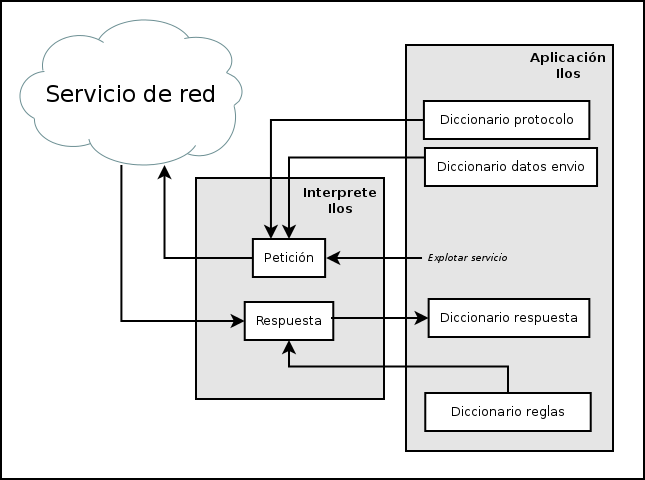
\includegraphics[scale=0.5]{img/service.png}
 \end{center}
 
 \caption{Arquitectura comunicación} 
 \label{fig:arquitectura}
 \end{figure}  
 
Los diccionarios de protocolo y datos de envío se utilizan para llevar a cabo una petición al servicio descrito. Mediante el diccionario de 
reglas de transformación se declara la forma del diccionario final, y la forma de obtenerlo a partir de la respuesta original.    

Esta arquitectura de comunicación será estándar indistintamente del protocolo de red usado. Aunque cada uno definirá sus 
parámetros de configuración y la forma en la que se escribirán y aplicarán las reglas.

A la hora de definir las reglas de transformación Ilos puede parecer un lenguaje de ontologías ya que se basa en la 
formulación de un esquema conceptual que facilita la comunicación. En el sentido extricto de la definición, una ontología
ha de veerse como un entendimiento común y compartido de un dominio.  Los servicios usan lenguajes de ontologías para 
publicar datos interpretables por aplicaciones informáticas (web semántica). El lenguaje de ontologías establece el esquema 
sintáctico y semántico de los datos publicados. En este sentido Ilos no es exactamente un lenguaje de ontología
ya que la interpretación que se realiza del dominio es personalizado e interno al programa.  

Muchos servicios web disponen de una descripción ontológica de los datos y el dominio que modelan para que puedan
ser utilizados por otras aplicaciones. Un programa Ilos podrá utilizar esas ontologías como parte de las
reglas de transformación para obtener el diccionario resultado.

Ilos dispone de una función del lenguaje denominada conexión (representada por @), que es definida para cada protocolo 
y que a partir de los diccionarios descritos, realiza una conexión, obtiene los datos y devuelve el diccionario resultado.    

Como puede verse Ilos ofrece mecanismos para llevar a cabo una comunicación a alto nivel con el servicio, en el sentido de que
se hace una conversión de los datos a unas estructuras conocidas y con significado. No obstante para cada protocolo también 
permite establecer una conexión a bajo nivel, en la que no se realice una interpretación de los datos.

A pesar de que Ilos abstrae el proceso de comunicación con el servicio e interpretación los datos de respuesta, esto no lo logra de forma completa. El programador
debe conocer la respuesta original del servicio para expresar las reglas de transformación. No obstante Ilos puede aplicar algoritmos de inteligencia artificial 
a los datos originales para obtener el diccionario resultado. Así el diccionario de reglas no indicará cómo obtener los datos, y su uso quedará solo para indicar qué 
datos se quiere obtener. En este contexto se puede ver que Ilos podría ser un lenguaje en parte declarativo. 

La red está en constante cambio, los servicios evolucionan y modifican la estructura de los datos ofrecidos. Para ser efectivo Ilos debe proporcionar mecanismos para detectar y adaptarse 
al cambio. Mientras los conceptos representados no cambien significativamente es posible utilizar técnicas de inteligencia artificial sobre datos obtenidos con anterioriadad para
adaptarse al cambio. 

\section{Tipo de dato unificado}
En Ilos toman gran importancia los diccionarios. En este lenguaje el tipo de dato utilizado como base para modelar cualquier aspecto 
es el diccionario. 

En Ilos el concepto de diccionario esta ampliado: toda función ligada a una clave puede acceder de forma local a 
todos las claves del diccionario. Esto hace posible que se puedan ver los diccionarios como objetos que encapsulan tanto 
datos como funcionalidad. Incluso se puede definir relaciones entre objetos creando diccionarios anidados.

Todas los operadores y funciones del lenguaje están sobrecargados para tratar con diccionarios, la mayoría
de estas también devolverán elementos de este tipo. Esto hace posible que el programador no tenga que preocuparse
en gran medida de la estrucutra de los datos con los que opera.

Las comunicaciones con los servicios de red se modelan con diccionarios y producen como resultado un diccionario.

También se puede buscar patrones en cadenas de texto utilizando expresiones regular en un diccionario. Incluso las correspondencias
encontradas se presentarán en forma de diccionario.

Con diccionarios también se modelan las tablas de una base de datos y sus relaciones. De esta forma es fácil insertar 
datos en varias tablas con una única estructura de diccionarios anidados. Las consultas a la base de datos también producen y se definen a partir de diccionarios.

Ilos presenta características de los lenguajes de programación de arrays, ya que generaliza las operaciones escalares para que se puedan aplicar 
a arrays, en este caso diccionarios. Incluso las funciones definidas por el programador pueden ser llamadas desde un contexto para todo, de forma que se aplique a
todo un diccionario.
 

\section{El interprete}
Las instrucciones que conforman un programa Ilos se pueden escribir y organizar en uno o varios fichero de texto plano   

\subsection{Multinterprete}

\subsection {Control de errores}

\section{Uso de memoria}
En la ejecución de programa Ilos la memoria se puede dividir en tres zonas. Una primera denominada memoria de interprete que guarda las instrucciones
correspondientes al interprete del lenguaje. 



\section{Extendiendo el lenguaje}

\section{Personalizando el lenguaje}

\section {Usos de Ilos}

\section{Ejemplo de programa que explota un servicio web}
\begin{lstlisting}[language=bash]
#!/bin/ilos
insert (
  @(
    @des: {
      {
        title: @sel(".title p"),
        content: @sel(".content"),
        image: f(){
          return @(
            @des : { @sel(".imgs") },
            @con : @sel (".notice_imgs a [href]")
          );
        }
      }
    },
    @con: {
      url: "http://www.service.com/notice",
      method: "POST",
      data: {
        id : {0,1000},
      }
    },
    @ok (){
      @r = {
        @notices : merge(@r)
      }
    }
  )
);
\end{lstlisting}
\section{Licencias}

\section{Planificación}

\section{Herraminetas de desarrollo}


\end{document}
%%%%%%%%%%%%%%%%%%%%%%%%%%%%%%%%%%%%%%%%%%%%%%%%%%%%%%%%%%%%%%%%%%%%%%%%
%Fco. Javier Bohórquez Ogalla
